\documentclass[
  bibliography=totoc,     % Literatur im Inhaltsverzeichnis
  captions=tableheading,  % Tabellenüberschriften
  titlepage=firstiscover, % Titelseite ist Deckblatt
]{scrartcl}

% Paket float verbessern
\usepackage{scrhack}

% Warnung, falls nochmal kompiliert werden muss
\usepackage[aux]{rerunfilecheck}

% unverzichtbare Mathe-Befehle
\usepackage{amsmath}
% viele Mathe-Symbole
\usepackage{amssymb}
% Erweiterungen für amsmath
\usepackage{mathtools}

% Fonteinstellungen
\usepackage{fontspec}
% Latin Modern Fonts werden automatisch geladen
% Alternativ:
%\setromanfont{Libertinus Serif}
%\setsansfont{Libertinus Sans}
%\setmonofont{Libertinus Mono}
\recalctypearea % Wenn man andere Schriftarten gesetzt hat,
% sollte man das Seiten-Layout neu berechnen lassen

% deutsche Spracheinstellungen
\usepackage{polyglossia}
\setmainlanguage{german}
%test

\usepackage[
  math-style=ISO,    % ┐
  bold-style=ISO,    % │
  sans-style=italic, % │ ISO-Standard folgen
  nabla=upright,     % │
  partial=upright,   % ┘
  warnings-off={           % ┐
    mathtools-colon,       % │ unnötige Warnungen ausschalten
    mathtools-overbracket, % │
},                       % ┘
]{unicode-math}

% traditionelle Fonts für Mathematik
\setmathfont{Latin Modern Math}
% Alternativ:
%\setmathfont{Libertinus Math}

\setmathfont{XITS Math}[range={scr, bfscr}]
\setmathfont{XITS Math}[range={cal, bfcal}, StylisticSet=1]

% Zahlen und Einheiten
\usepackage[
locale=DE,                   % deutsche Einstellungen
separate-uncertainty=true,   % immer Fehler mit \pm
per-mode=symbol-or-fraction, % / in inline math, fraction in display math
]{siunitx}

% chemische Formeln
\usepackage[
version=4,
math-greek=default, % ┐ mit unicode-math zusammenarbeiten
text-greek=default, % ┘
]{mhchem}

% richtige Anführungszeichen
\usepackage[autostyle]{csquotes}

% schöne Brüche im Text
\usepackage{xfrac}

% Standardplatzierung für Floats einstellen
\usepackage{float}
\floatplacement{figure}{htbp}
\floatplacement{table}{htbp}

% Floats innerhalb einer Section halten
\usepackage[
section, % Floats innerhalb der Section halten
below,   % unterhalb der Section aber auf der selben Seite ist ok
]{placeins}

% Seite drehen für breite Tabellen: landscape Umgebung
\usepackage{pdflscape}

% Captions schöner machen.
\usepackage[
  labelfont=bf,        % Tabelle x: Abbildung y: ist jetzt fett
  font=small,          % Schrift etwas kleiner als Dokument
  width=0.9\textwidth, % maximale Breite einer Caption schmaler
]{caption}
% subfigure, subtable, subref
\usepackage{subcaption}

% Grafiken können eingebunden werden
\usepackage{graphicx}
% größere Variation von Dateinamen möglich
\usepackage{grffile}

% schöne Tabellen
\usepackage{booktabs}

% Verbesserungen am Schriftbild
\usepackage{microtype}

% Literaturverzeichnis
\usepackage[style=alphabetic,]{biblatex}
% Quellendatenbank
\addbibresource{lit.bib}
\addbibresource{programme.bib}

% Hyperlinks im Dokument
\usepackage[
  unicode,        % Unicode in PDF-Attributen erlauben
  pdfusetitle,    % Titel, Autoren und Datum als PDF-Attribute
  pdfcreator={},  % ┐ PDF-Attribute säubern
  pdfproducer={}, % ┘
]{hyperref}
% erweiterte Bookmarks im PDF
\usepackage{bookmark}

% Trennung von Wörtern mit Strichen
\usepackage[shortcuts]{extdash}

\title{V46: Faraday-Effekt an Halbleitern}
\author{
  Martin Schönfeld
  \texorpdfstring{
    \\
    \href{mailto:martin.schoenfeld@udo.edu}{martin.schoenfeld@udo.edu}
  }{}
  \texorpdfstring{\and}{, }
  Tim Sedlaczek
  \texorpdfstring{
    \\
    \href{mailto:tim.sedlaczek@udo.edu}{tim.sedlaczek@udo.edu}
  }{}
}
\publishers{TU Dortmund – Fakultät Physik}

\date{Durchführung: 17.10.2022\\
      Abgabe: 28.10.2022}


\begin{document}

\maketitle
\thispagestyle{empty}
\setcounter{page}{1}
\pagenumbering{arabic} 

\section{Zielsetzung}
\label{sec:Zielsetzung}

Das Ziel dieses Versuchs ist es, die effektive Masse von Leitungselektronen in
GaAs zu ermitteln.
Es wird dazu die Faraday-Rotation an unterschiedlich stark
dotierten Proben für verschiedene Wellen gemessen.

\section{Theorie}
\label{sec:Theorie}

\subsection{Die effektive Masse}
\label{sec:effMasse}
Die Bandstruktur von Halbleitern ist kompliziert. 
In der Nähe des Minimums des
Leitungsbands am Punkt $\vec{k} = \vec{0}$ kann die $E\left(\vec{k}\right)$-
Relation in eine Taylorreihe zu
\begin{equation*}
  E\left(\vec{k}\right) = E_\text{0} +
  \frac{1}{2} \sum_{i = 1}^3
  \left(\frac{\partial^2 E}{\partial k_\text{i}^2}\right)_{\vec{k} = \vec{0}}
  k_\text{i} + ...
\end{equation*}
entwickelt werden.
Hier steht $\vec{k}$ für den Wellenvektor des Elektrons und der Index
$i$ steht für die Raumdimensionen.
Diese Taylorreihe wird in die parabolische Relation eines freien Elektrons
überführt, wobei
\begin{equation}
  m_\text{i}^* := \hbar^2
  \left(\frac{\partial^2 E}{\partial k_\text{i}^2}\right)_{\vec{k} = \vec{0}}^{-1}
  \label{eqn:effMasse}
\end{equation}
die effektive Masse definiert.
Hierbei ist $\hbar$ das reduzierte Plancksche Wirkungsquantum.
Durch Substitution der Elektronenmasse durch die effektive Masse lässt
sich somit für Leitungselektronen die Quantenmechanik freier Teilchen
anwenden. Dabei ist der Einfluss des Kristallpotentials berücksichtigt.

\subsection{Rotation linear polarisierten Lichts in doppelbrechenden Kristallen}
\label{sec:Theo1}
Wenn links- und rechtszirkular polarisiertes Licht linear überlagert wird,
lässt sich dies als linear polarisiertes Licht verstehen.
Die Phasengeschwindigkeiten beider zirkularer Wellen werden beim Durchlaufen
eines doppelbrechenden Kristalls der Länge $L$ unterschiedlich. Damit wird
die lineare Polarisationsrichtung gedreht um einen Winkel
\begin{equation}
  \theta = \frac{L}{2} \left(\vec{k_\text{R}} - \vec{k_\text{L}}\right) .
  \label{eqn:Winkel-2}
\end{equation}
Dabei beschreibt $\vec{k_\text{R}}$ den Wellenvektor des rechtszirkular und
$\vec{k_\text{L}}$ den Wellenvektor des linkszirkular polarisierten Lichts.
Mittels elektrischer Dipole lässt sich dieser Effekt erklären, diese werden
im Kristall induziert.
In einem externen elektrischen Feld $\vec{E}$ werden zum einen positive Ionen relativ
zu negativen Ionen verschoben, oder zum anderen der Ladungsschwerpunkt der
positiven Ladungen und der Elektronenverteilung stimmt nicht überein.
Die Summe der einzelnen Dipolmomente pro Volumen erzeugt eine Polarisation
\begin{equation}
  \vec{P} = \epsilon_0 \; \chi \; \vec{E}
  \label{eqn:Polarisation}
\end{equation}
mit der elektrischen Feldkonstanten $\epsilon_0$ und der
\emph{dielektrischen Suszeptibilität} $\chi$.
Dabei ist die Suszeptibilität $\chi$ im Allgemeinen ein Tensor.
Ein Material ist doppelbrechend, wenn im Suszeptibilitätstensor
nicht-diagonale und komplex konjugierte Koeffizienten auftreten.
Für in $z$-Richtung durchlaufendes Licht hat ein solcher Tensor
mit allen für die Drehung relevanten Koeffizienten die Gestalt
\begin{equation*}
  \chi =
  \begin{pmatrix}
    \chi_\text{xx} & i \chi_\text{xy} & 0 \\
    -i \chi_\text{xy} & \chi_\text{xx} & 0 \\
    0 & 0 & \chi_\text{zz} \\
  \end{pmatrix}
\end{equation*}
Ein Ausdruck für den Drehwinkel kann nun durch Einsetzen des Ansatzes
einer ebenen Welle in die Wellengleichung in Materie gewonnen werden.
Es ergeben sich nach Zerlegung in die Komponenten drei Gleichungen,
aus einer folgt $E_\text{z} = 0$.
% Es liegt also eine transversale Wellenausbreitung vor.
Für die beiden übrigen Gleichungen muss für eine nicht-trivial Lösung
\begin{equation*}
  \left(- k^2 + \frac{\omega^2}{c^2} \left(1 + \chi_\text{xy}\right)\right)^2
  -\left(i \frac{\omega^2}{c^2} \chi_\text{xy}\right)
  \left(- i \frac{\omega^2}{c^2} \chi_\text{xy}\right)
  = 0
\end{equation*}
mit der Lichtgeschwindigkeit $c$ und der Kreisfrequenz $\omega$
der Welle gelten.
Daraus folgen die zwei möglichen Wellenzahlen
\begin{equation*}
  k_\pm = \frac{\omega}{c} \sqrt{\left(1 + \chi_\text{xx}\right) \pm \chi_\text{xy}},
\end{equation*}
und wiederum daraus zwei Phasengeschwindigkeiten
% \begin{align*}
%   v_\text{Ph,R} &=
%   \frac{c}{\sqrt{1 + \chi_\text{xx} + \chi_\text{xy}}}\\
%   v_\text{Ph,L} &=
%   \frac{c}{\sqrt{1 + \chi_\text{xx} - \chi_\text{xy}}}\\
% \end{align*}
für eine rechts- beziehungsweise linkszirkular polarisierte Welle.
Daraufhin werden diese Wellenzahlen in den Ausdruck \eqref{eqn:Winkel-2}
eingesetzt und linearisiert, wodurch sich der der Ausdruck
\begin{equation}
  \theta \approx \frac{L \, \omega}{2 \, c \, n} \chi_\text{xy}
  \label{eqn:Winkel-1}
\end{equation}
mit Brechungsindex $n = c / v_\text{Ph}$ ergibt.


\subsection{Faraday-Rotation in optisch inaktiven Medien}
\label{sec:Theo22}
Die Polarisationsrichtung von Licht in einem optisch inaktiven Medium bleibt unverändert.
Geändert wird die Polarisationsrichtung Durch Anwesenheit eines externen magnetischen Feldes $\vec{B}$.
Dieses muss parallel zur Ausbreitungsrichtung des Lichts sein.
Durch die Gleichung
\begin{equation*}
  m_\text{e} \frac{\symup{d}^2 \vec{r}}{\symup{d} t^2} + K \, \vec{r} =
  - e_0 \vec{E}\left(r\right)
  - e_0 \frac{\symup{d} \vec{r}}{\symup{d} t} \times \vec{B}
\end{equation*}
wird ein Elektron beschrieben, wobei durch $m_\text{e}$ die Masse und $e_0$ die Ladung des Elektrons,
durch $K$ eine die Bindung beschreibende Konstante und durch
$\vec{E}$ die Feldstärke der einfallenden Lichtwelle darstellt.
Weiterhin wird angenommen, dass $\vec{E}$ harmonisch in der Zeit
oszilliert, die Polarisation $\vec{P}$ ist proportional zu $\vec{r}$
die Richtung des Magnetfeldes ist die z-Richtung, wodurch sich diese Gleichung
zerlegen lässt.
Nur für $E_\text{z} = 0$ ergeben sich nicht triviale Lösungen, wodurch sich die
Anzahl an Komponentengleichungen auf zwei reduziert.
Nun wird der Ansatz
\begin{equation*}
  \chi =
  \begin{pmatrix}
    \chi_\text{xx} & i \chi_\text{xy} & 0 \\
    i \chi_\text{yx} & \chi_\text{xx} & 0 \\
    0 & 0 & \chi_\text{zz} \\
  \end{pmatrix}
\end{equation*}
genutzt und setzt diesen in die verbleibenden zwei Komponenten von \eqref{eqn:Polarisation} ein.
Diese Gleichung wird nach Real- und Imaginärteil separiert, so ergibt sich
\begin{equation*}
  \chi_\text{xy} = - \chi_\text{yx}.
\end{equation*}
Also dreht sich die Polarisationsebene von einfallendem Licht in einem
optisch inaktiven Medium bei einem externen Magnetfeld parallel zur
Ausbreitungsrichtung, dies wird Faraday-Effekt genannt.
Der Drehwinkel lässt sich mit Gleichung \eqref{eqn:Winkel-1} und den zuvor genannten Überlegungen
wie folgt ausdrücken
\begin{equation*}
  \theta = \frac{e_0^3}{2 \epsilon_0 c}\frac{1}{m_\text{e}^2}
  \frac{\omega^2}{\left(-\omega^2 + \frac{K}{m_\text{e}}\right)^2 -
  \left(\frac{e_0}{m_\text{e}} B \omega\right)^2}
  \frac{N B L}{n}
\end{equation*}
Hierbei beschreibt $m_\text{e}$ die Masse des Elektrons und $N$
die Anzahl an Elektronen pro Volumen.
Die Zyklotronfrequenz $\omega_\text{Z} = B e_0 / m_\text{e}$ ist die Frequenz eines aufgrund
der Lorentzkraft im magnetischen Feld rotierenden Elektrons und $\omega_0 = \sqrt{K / m_\text{e}}$
ist die Resonanzfrequenz hat.
Der Grenzfall $\omega_0 \rightarrow 0$ ist erfüllt für quasifreie Ladungsträger
\begin{equation}
  \theta_\text{frei} \approx \frac{e_0^3}{8 \pi^2 \epsilon_0 c^3}
  \frac{1}{m_\text{e}^2} \lambda^2 \frac{N B L}{n}.
  \label{eqn:theta-frei}
\end{equation}
Sonst ist in Halbleitern die Resonanzfrequenz $\omega_0$
deutlich größer als die Zyklotronfrequenz, sodass folgende Näherungen getroffen werden können
\begin{equation*}
  \left(\omega_0^2 - \omega^2\right)^2 >> \omega^2 \omega_\text{Z}^2
  \text{    und    }
  \omega << \omega_0
\end{equation*}
Hierdurch ergibt sich die wichtige Relation
\begin{equation}
  \theta\left(\lambda\right) \approx \frac{2 \pi^2 e_0^3 c}{\epsilon_0}
  \frac{1}{m_\text{e}^2}\frac{1}{\lambda^2 \omega_0^4}
  \frac{N B L}{n}.
  \label{eqn:theta-gebunden}
\end{equation}

\newpage
\section{Versuchsaufbau}
\label{sec:Aufbau}

Der in Abbildung \ref{fig:Aufbau} dargestellte Versuchsaufbau wird verwendet, um
die Faraday-Rotation zu messen.

\begin{figure}
  \centering
  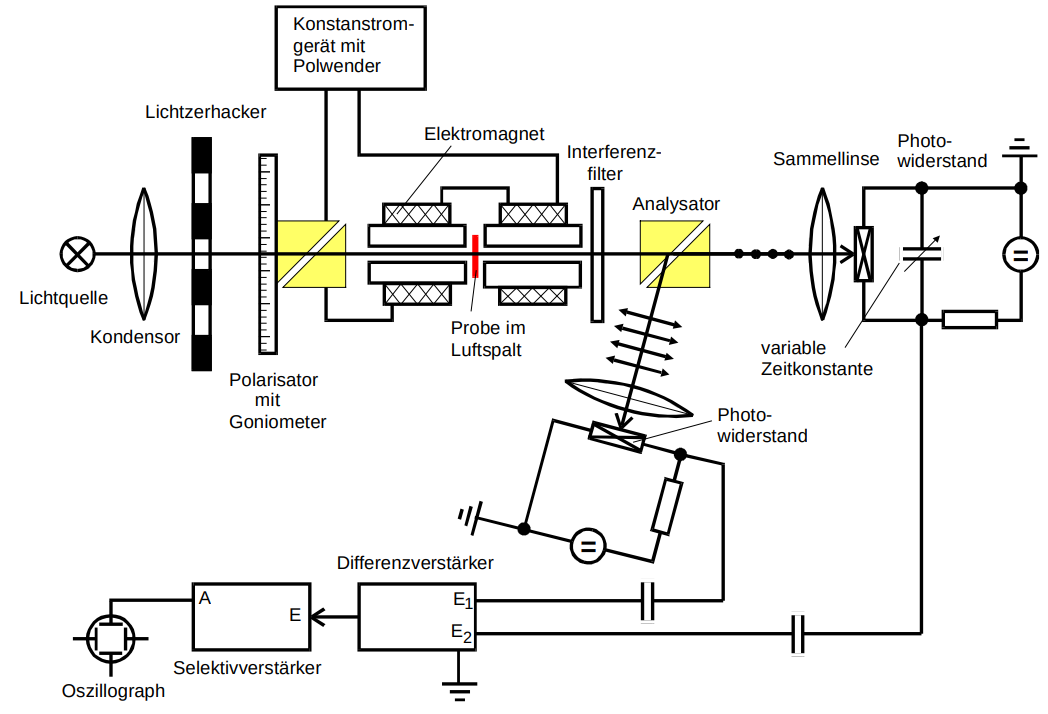
\includegraphics[width=\textwidth]{images/aufbau.png}
  \caption{Der für die Messung verwendete Versuchsaubau in schematischer Darstellung \cite{anleitung}.}
  \label{fig:Aufbau}
\end{figure}
\noindent
Eine Halogenlampe spendet Licht, welches mit einem Kondensor bzw. einer Sammellinse parallelisiert
wird. Anschließend wird dieses Licht mit einem Lichtzerhacker frequentiert.
Die Amplitude des Lichtsignals oszilliert somit in der Frequenz des
Lichtzerhackers. Danach fällt der Lichtstrahl auf ein Glan-Thomson
Prisma, welches das Licht linear polarisiert.
Der Drehwinkel des Polarisators ist ablesbar an einem Goniometer.
Dieses linear polarisierte Licht läuft danach durch einen Elektromagneten.
Dort befindet sich die zu untersuchende Probe in einem Luftspalt.
Das externe Magnetfeld wird durch ein Konstantstromgerät erzeugt
und an die Probe angelegt.
Das Licht wird hinter dem Magnetfeld mit einem Interferenzfilters monochromatisiert.
Der Aufbau des Interferenzfilters ergibt sich aus einem Dielektrikum zwischen zwei
transparenten Scheiben. An diesen werden die Lichtstrahlen an jeder
Schicht teilweise reflektiert. Eine Transmission ergibt sich lediglich, wenn bei
den Teilstrahlen konstruktive Interferenz gegeben ist.
Es ergibt sich jedoch nur eine Verteilung endlicher Breite und keine scharfe Spitze.
Das liegt an der begrenzten Anzahl an Schichten, die reflektieren.
Das annähernd monochromatische Licht trifft danach auf ein zweites Glan-Thomson-Prisma.
Dieses teilt den Lichstrahl in zwei orthogonal zueinander linear polarisierte
Lichstrahlen. Diese beiden Strahlen werden dann mit Hilfe einer Sammellinse
auf einen Photowiderstand fokussiert, welche sich in einem geerdeten Schaltkreis
befinden und dort mit einem Vorwiderstand und einer Spannungsquelle verbunden sind.
Die Photowiderstände bestehen aus amorphen PbS Halbleitern.
% amorph: Keine Fernordnung, aber Nahordnung. => Unregelmäßige Muster
Die Intensität des Lichts bestimmt, wie viele Elektronen aus dem Halbleiter
rausgelöst werden. Dies geschieht über den äußeren Photoeffekt.
Die so im Halbleitermaterieal entstehenden Löcher werden mit Elektronen 
aus dem Schaltkreis wieder aufgefüllt. Genau das ist messbar durch einen Abfall
an dem Widerstand der Spannung. Dieser Innenwiderstand
ist proportional zur Lichtintensität \cite{anleitung}.
Die an den Photowiderständen abfallende Wechselspannung wird ausgekoppelt 
auf Kondensatoren, die an einem Differenzverstärker angeschlossen sind.
Eine regelbare Zeitkonstante befindet sich parallel zum Photowiderstand
geschaltet im Schaltkreis, um den Strahlengang zu messen.
Hierdurch wird eine Anpassung der Phase an das Signal des anderen 
Photowiderstands ermöglicht.
Die Charakteristik des Differenzverstärkers ist es, die Differenz der beiden
Wechselspannungen abzubilden. Dies wird an einen Selektivverstärker weitergegeben.
Ein Selektivverstärker ähnelt einem Bandpass mit regelbarer
Frequenz. Dieser filtert alle Frequenzen außer der eingestellten Frequenz raus.
Letztendlich wird das gefilterte Signal auf einem Oszilloskop angezeigt.

\section{Durchführung}
\label{sec:Durchführung}

\subsection{Kalibrierung des Aufbaus}
\label{sec:Kalibrierung}
Zuerst muss der Versuchsaufbau justiert werden. Dafür werden die Halogenlampe,
Kondensor, Lichtzerhacker, Polarisator, Elektromagnet, Analysator und die beiden
Photowiderstände so positioniert, dass beide Photowiderstände vom Licht getroffen
werden. Hierfür werden die Deckel der Photowiderstandsgehäuse entfernt. 
Daraufhin ist das Ziel, dass der durchgehende Strahl verschwindet. Dafür
wird das Analysatorprisma um seine vertikale Achse gedreht.
Daraufhin wird der Lichtzerhacker eingestellt. %hier
Zur Ermittlung der Frequenz wird der Photowiderstand des durchgehenden
Strahles an das Oszilloskop angeschlossen und die Frequenz abgelesen.
Nun wird eine der Proben in den Luftschacht des Elektromagneten installiert und
die Photowiderstände werden an die Eingänge des Differenzverstärkers angeschlossen.
Daraufhin wird der Ausgang des Differenzverstärkers mit dem Eingang des
Selektivverstärkers verbunden.
Letztlich wird der Ausgang des Selektivverstärkers an das Oszilloskop
angeschlossen.

\subsection{Vermessung der Faraday-Rotation}
\label{sec:MessungFaraday}

Um die tatsächliche Faraday-Rotation zu messen, wird die Konstantstromquelle
auf das Maximum von \SI{10}{\ampere} eingestellt. Das Magnetfeld ist nun
hergestellt und in das Magnetfeld werden für acht verschiedene Interferenzfilter
jeweils drei Proben in den Luftspalt eingesetzt. Dann wird für jeden
Fliter das beobachtete Signal am Oszilloskop auf ein Minimum abgeglichen.
Hierzu wird der Polarisator gedreht. Der Winkel des Polarisators wird mit einem
Gonoimeter abgelesen und für jeden Filter notiert. 
Danach wird das Magnetfeld umgepolt und die gleiche Messung durchgeführt.
Die verwendeten Proben sind
\begin{enumerate}
  \item n-dotiertes GaAs mit
  $N = \SI{2.8e18}{\raiseto{-3}\centi\meter}$ und
  $L = \SI{1.296}{\milli\meter}$
  \item n-dotiertes GaAs mit
  $N = \SI{1.2e18}{\raiseto{-3}\centi\meter}$ und
  $L = \SI{1.36}{\milli\meter}$
  \item hochreines GaAs mit
  $L = \SI{5.11}{\milli\meter}$
\end{enumerate}
Die Interferenzfilter sind jewwils für die Wellenlängen
\SI{1060}{\nano\meter}, \SI{1290}{\nano\meter}, \SI{1450}{\nano\meter}, \SI{1720}{\nano\meter}, \SI{1960}{\nano\meter}, 
\SI{2156}{\nano\meter}, \SI{2340}{\nano\meter}, \SI{2510}{\nano\meter} und \SI{2650}{\nano\meter} durchlässig.

\subsection{Messung der magnetischen Flussdichte der Spule}
\label{sec:MessungBFeld}

Das angelegte magnetische Feld, in dem sich die Probe befindet wird
mit Hilfe einer Hall-Sonde gemessen.
Hierfür wird das Konstantstromgerät auf den
maximalen Strom von ungefähr \SI{10}{\ampere} eingestellt. Mit der
Spitze der Hall-Sonde wird daraufhin der Luftspalt abgefahren.
In Abständen von \SI{1}{\milli\meter} wird dann die magnetische Flussdichte vermessen.

\section{Auswertung}
\label{sec:Auswertung}

\subsection{Bestimmung der maximalen magnetischen Flussdichte $|\vec{B}|_\text{max}$}

In der Probenkammer wird in Strahlrichtung abhängig vom Ort $z$ die magnetische Flussdichte $|\vec{B}(z)| = B(z)$
gemessen. Diese sind in Tabelle \ref{tab:messwerte_hall} zu sehen. Diese Messwerte werden in \ref{fig:feldmessung2} mit
Hilfe von

\begin{equation}
    B(z) = a \cdot z^4 + b \cdot z^3 + c \cdot z^2 + d \cdot z + e
\end{equation}
approximiert aufgetragen. Dies wird durchgeführt mit Hilfe der Funktion \textit{scipy.optimize.curve\_fit} aus der Python-Bibliothek SkiPy.
$z$ ist dabei relativ von der ungefähren Probenmitte gemessen, diese befindet sich bei $z = \SI{130}{\milli\metre}$.
Es ergeben sich die Approximationsparameter

\begin{align*}
    a &= \SI{-0.00218 +- 0.00103}{\milli\tesla\per\milli\meter\tothe{4}} \\
    b &= \SI{ 0.00958 +- 0.00749}{\milli\tesla\per\milli\meter\tothe{3}} \\
    c &= \SI{-1.68080 +- 0.17851}{\milli\tesla\per\milli\meter\tothe{2}} \\
    d &= \SI{ 1.86273 +- 0.93305}{\milli\tesla\per\milli\meter}          \\
    e &= \SI{ 430.829 +- 5.55488}{\milli\tesla} \; .
\end{align*}
Zur Bestimmung des Maximums der Fitkurve wird die Nullstelle der ersten Ableitung bestimmt durch

\begin{equation}
    B'(z) = 4a \cdot z^3 + 3b \cdot z^2 + 2c \cdot z + d \stackrel{!}{=} 0.
\end{equation}
Es ergibt sich $z_\text{max} = \SI{0.56}{\milli\meter}$ und die maximale magnetische Flussdichte

\begin{equation*}
    B_\text{max} = |B(z_\text{max})| = \SI{431.347}{\milli\tesla}.
\end{equation*}
Dies ist ersichtlich in Abbildung \ref{fig:feldmessung2}.
\begin{figure}[H]
    \centering
    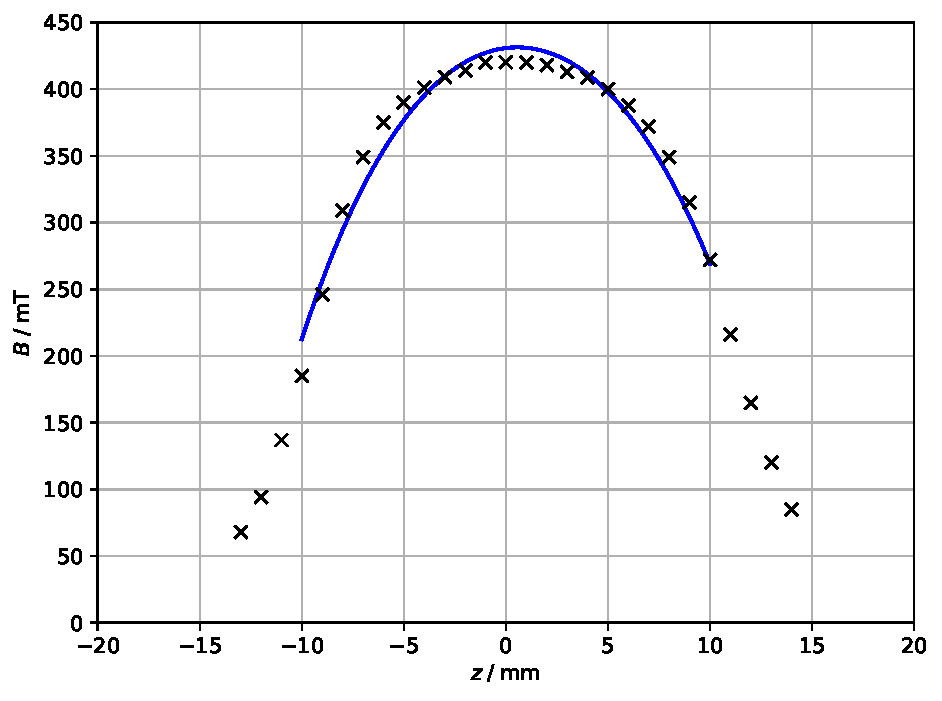
\includegraphics[scale=0.8]{build/feldmessung2.pdf}
    \caption{Messwerte der magnetischen Feldstärke $B(z)$ in Abhängigkeit des Ortes $z$, genähert um den Hochpunkt}
    \label{fig:feldmessung2}
\end{figure}

\begin{table}[h]
    \footnotesize
    \centering
    \caption{Mit einer Hall-Sonde gemessene Magnetfeldstärke im Bereich des Luftspalts zur Bestimmung des Maximalwerts.}
    \label{tab:messwerte_hall}
    \begin{tabular}{S[table-format=1.1] S S S S}
      {$z$ / mm} & {$B$ / mT} & {$z$ / mm} & {$B$ / mT} \\
      \midrule
      104 & 0 & 132 & 418 \\
      105 & 1 & 133 & 413 \\
      106 & 2 & 134 & 409 \\
      107 & 2 & 135 & 400 \\
      108 & 3 & 136 & 388 \\
      109 & 5 & 137 & 372 \\
      110 & 7 & 138 & 349 \\
      111 & 9 & 139 & 315 \\
      112 & 13 & 140 & 272 \\
      113 & 18 & 141 & 216 \\
      114 & 25 & 142 & 165 \\
      115 & 34 & 143 & 120 \\
      116 & 48 & 144 & 85 \\
      117 & 68 & 145 & 61 \\
      118 & 94 & 146 & 43 \\
      119 & 137 & 147 & 31 \\
      120 & 185 & 148 & 23 \\
      121 & 246 & 149 & 16 \\
      122 & 309 & 150 & 12 \\
      123 & 349 & 151 & 9 \\
      124 & 375 & 152 & 6 \\
      125 & 390 & 153 & 5 \\
      126 & 401 & 154 & 3 \\
      127 & 409 & 155 & 2 \\
      128 & 414 & 156 & 2 \\
      129 & 420 & 157 & 1 \\
      130 & 420 & 158 & 1 \\
      131 & 420 & 159 & 0 \\
    \end{tabular}
  \end{table}

\subsection{Bestimmung der effektiven Masse von $\ce{GaAs}$}

Zur Bestimmung der effektiven Massen der hochreinen und n-dotierten $\ce{GaAs}$-Proben, werden die in den 
Tabellen \ref{tab:mess2}, \ref{tab:mess3} und \ref{tab:mess4} aufgelisteten Daten der Faradayrotation

\begin{equation}
    \theta = \frac{1}{2} (\theta_1 - \theta_2)
\end{equation}
zusammen mit den Probendicken $d$ normiert.
Die Probendicken waren angegeben zu

\begin{align*}
    d_\text{hochrein} &= \SI{5.11}{\milli\meter} \\
    d_{N = \SI{2.8e18}{\per\cubic\centi\meter}} &= \SI{1.296}{\milli\meter} \\
    d_{N = \SI{1.28e18}{\per\cubic\centi\meter}} &= \SI{1.36}{\milli\meter} \; .
\end{align*}
Die Faradayrotationen $\sfrac{\theta}{d}$ sind normiert in Abbildung \ref{fig:plot2} gegen $\lambda^2$ aufgetragen.
Die Faradayrotationen der hochreinen Probe werden von den normierten Faradayrotationen der n-dotierten Proben
abgezogen.
Für die Regressionsparameter für die Proben mit $N = \SI{2.8e18}{\per\cubic\centi\meter}$ und 
$\SI{1.28e18}{\per\cubic\centi\meter}$ ergibt sich:

\begin{align*}
    a_1 &= \SI{14.62 +- 1.32}{\meter\tothe{-3}}\\
    a_2 &= \SI{6.91 +- 0.77}{\meter\tothe{-3}}\; .
\end{align*}
Die effektiven Massen 

\begin{equation}
    m^* = \sqrt{\frac{e_0^3}{8\pi^2\epsilon_0 c^3} \frac{NB_\text{max}}{n} \frac{1}{a}}
\end{equation}
ergeben sich mit einem Brechungsindex von $n = \num{3.5}$ zu 
 
\begin{align*}
    m^*_{1,N = \SI{2.8e18}{\per\cubic\centi\meter}} &= \num{0.0776} \cdot m_e \\
    m^*_{2,N = \SI{1.28e18}{\per\cubic\centi\meter}} &= \num{0.0765} \cdot m_e 
\end{align*}
relativ zur Elektronenmasse $m_e = \SI{9.1093837015e-31}{\kilo\gram}$.


\begin{figure}[H]
    \centering
    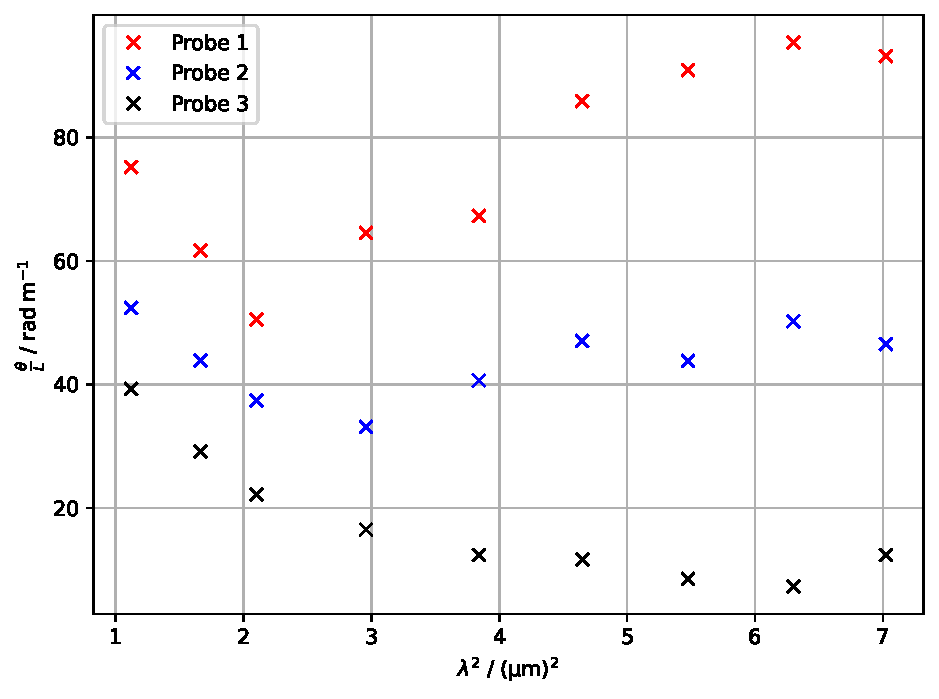
\includegraphics[scale=0.7]{build/winkel.pdf}
    \caption{Normierte Faradayrotationen $\sfrac{\theta}{d}$ der drei Proben aufgetragen gegen $\lambda^2$}
    \label{fig:plot2}
\end{figure}

\begin{table}
    \centering
    \caption{Winkelmesswerte in Abhängigkeit der gefilterten Lichtwellenlänge $\lambda$ 
        der hochreinen $\ce{GaAs}$-Probe}
    \label{tab:mess2}
    \sisetup{table-format=2.1}
    \begin{tabular}{c c c c c}
    \toprule
    $\lambda \;/\; \si{\micro\meter}$ & $\theta_1 \;/\; \si{\degree}$ &  $\theta_2 \;/\; \si{\degree}$\\
    \midrule
        1,06 & 273,00 & 250,00 \\
        1,29 & 269,11 & 252,00 \\
        1,45 & 268,64 & 255,64 \\
        1,72 & 266,32 & 256,64 \\
        1,96 & 260,83 & 253,58 \\
        2,16 & 260,00 & 253,16 \\
        2,34 & 233,50 & 228,50 \\
        2,51 & 214,33 & 210,08 \\
        2,65 & 164,90 & 157,39 \\
    \bottomrule
    \end{tabular}
\end{table}

\begin{table}
    \centering
    \caption{Winkelmesswerte in Abhängigkeit der gefilterten Lichtwellenlänge $\lambda$ 
        der n-dotierten $\ce{GaAs}$-Probe mit $N = \SI{2.8e18}{\per\cubic\centi\meter}$}
    \label{tab:mess3}
    \sisetup{table-format=2.1}
    \begin{tabular}{c c c c c}
    \toprule
    $\lambda \;/\; \si{\micro\meter}$ & $\theta_1 \;/\; \si{\degree}$ &  $\theta_2 \;/\; \si{\degree}$\\
    \midrule
        1,06 & 268.83 & 257.67 \\ 
        1,29 & 266.17 & 257.00 \\
        1,45 & 266.33 & 258.84 \\
        1,72 & 266.08 & 256.50 \\ 
        1,96 & 263.00 & 253.00 \\ 
        2,16 & 263.33 & 250.67 \\ 
        2,34 & 238.50 & 225.00 \\ 
        2,51 & 220.83 & 206.66 \\ 
        2,65 & 167.08 & 153.25 \\ 
    \bottomrule
    \end{tabular}
\end{table}

\begin{table}
    \centering
    \caption{Winkelmesswerte in Abhängigkeit der gefilterten Lichtwellenlänge $\lambda$ 
        der n-dotierten $\ce{GaAs}$-Probe mit $N = \SI{1.2e18}{\per\cubic\centi\meter}$}
    \label{tab:mess4}
    \sisetup{table-format=2.1}
    \begin{tabular}{c c c c c}
    \toprule
    $\lambda \;/\; \si{\micro\meter}$ & $\theta_1 \;/\; \si{\degree}$ &  $\theta_2 \;/\; \si{\degree}$\\
    \midrule
        1,06 & 266.83 & 258.00 \\ 
        1,29 & 263.16 & 257.00 \\
        1,45 & 265.00 & 259.16 \\
        1,72 & 263.33 & 258.16 \\
        1,96 & 259.67 & 253.33 \\
        2,16 & 259.17 & 251.83 \\
        2,34 & 233.00 & 226.17 \\
        2,51 & 216.00 & 208.17 \\
        2,65 & 166.33 & 159.08 \\
    \bottomrule
    \end{tabular}
\end{table}


\begin{figure}[H]
    \centering
    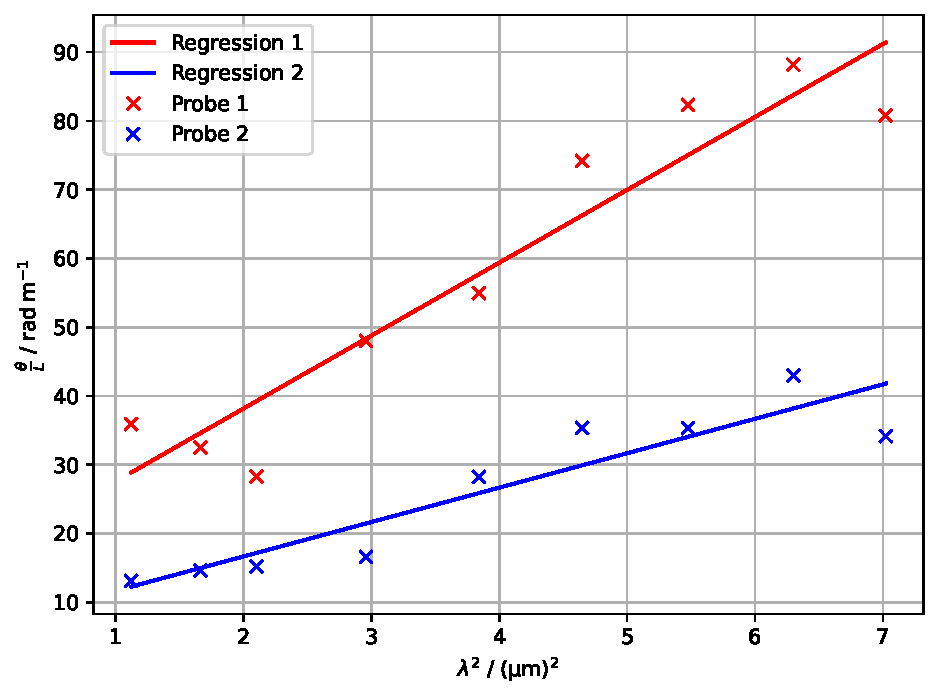
\includegraphics[scale=0.7]{build/differenzen.pdf}
    \caption{Lineare Approximationen der beiden Differenzen der normierten Faradayrotation $\sfrac{\theta}{d}$ 
              der hochreinen $\ce{GaAs}$-Probe von denen der n-dotierten Proben, aufgetragen gegen $\lambda^2$}
    \label{fig:plot3}
  \end{figure}

  \newpage
  \section{Diskussion}
  \label{sec:Diskussion}
  
  Das vermessene Magnetfeld ist in Anbetracht der Dicke der Proben relativ
  homogen.
  Für die beiden verwendeten Proben ergeben sich Theoriewerte von
  \begin{align*}
    \frac{m^*_1}{m_\text{e}} &\approx \num{0.0778} \\
    \frac{m^*_2}{m_\text{e}} &\approx \num{0.0765}.
  \end{align*}
  Es zeigen sich Abweichungen von Werten um 16\% zum Vergleich mit dem 
  Theoriewert \cite[3]{effmasse}. Dies lässt sich auf mehrere Ursachen zurückführen:
  Das Signal am Oszilloskop konnte nicht auf Null runtergeregelt werden. 
  Wegen dieses Rauschens war eine präzise Einstellung mit dem Goniometer
  nicht gut möglich. Aus diesem Grund können die Steigungen der Regressionen
  und somit auch die effektive Masse nur ungenau bestimmt werden.
  Durch Wärmestrahlung lässt sich das Rauschen des Signals teilweise 
  erklären, welche die Spule und die Proben aufgrund des Aufheizens im Laufe
  der Messung emittieren.
  Außerdem sind die Verstaubung der Filter sowie die Fingerabdrücke auf den
  Proben erwähnenswert, die zu weiteren Störungen geführt haben können.
  Die Messung und Auswertung für die Bestimmung des Maximalwerts des 
  Magnetfeldes zeigt, dsas die gewählte Ausgleichsfunktion mit einer
  vierten Potenz eine gute Näherung liefert.

  \newpage 
  \printbibliography 
\end{document}